\section{Creating a guide}\label{sec:Creating_a_guide}
\subsubsection*{Context} Meaning-carrying tools, like handbooks or maps, can help collect content and stories as well as assist others who want to adopt the idea.

\subsubsection*{Problem} 
Established ideas have knowledge cartography challenges for newcomers, consider trying to decipher a subway map in a foreign city. When the idea or system is only ``newly discovered'', the associated meanings may not be well understood, and indeed they may not have been created. Even if a topic is only ``personally new'', it can be hard to find one's way around.

\subsubsection*{Solution}
The process of creating the guide can go hand-in-hand with figuring out how the system works. Thus, techniques of \href{http://knowledgecartography.org/}{knowledge cartography} and \href{http://www.hitl.washington.edu/publications/r-97-47/two.html}{meaning making} are useful for would-be guide creators.\footnote{We started the Peeragogy project by collaboratively making an outline for the Peeragogy Handbook. We recommended this
handbook-making practice to others, as a way to learn collaboratively and build a strong group.}

\subsubsection*{Rationale} 
It is important to keep in mind how ``the map is not the territory,'' and map-making is only one facet of shared human activity. For instance, a pattern description can be thought of as a ``micro-map'' of a specific activity. These maps are not useful if they are divorced from practice. The process of creating a guide creates a certain formality to the project, forcing participants to catalogue and explicate their idea. Additionally, the act generally leads to deadlines which can help prod individuals to work on the project more regularly.

\subsubsection*{Resolution}
Writing down this pattern clarifies the importance of creating a guide for your idea if you want others to adopt it for use.\footnote{As \href{https://www.gnu.org/philosophy/free-doc.html}{Richard Stallman} wrote about free software documentation: ``The biggest deficiency in free operating systems is not in the software—it is the lack of good free manuals that we can include in these systems. The biggest deficiency in free operating systems is not in the software—it is the lack of good free manuals that we can include in these systems. Many of our most important programs do not come with full manuals. Documentation is an essential part of any software package; when an important free software package does not come with a free manual, that is a major gap.''}  If people complain that they are confused, now we know why.

\subsubsection*{What's Next} 
Working with our shepherd at PLoP to improve this paper!


\begin{figure}
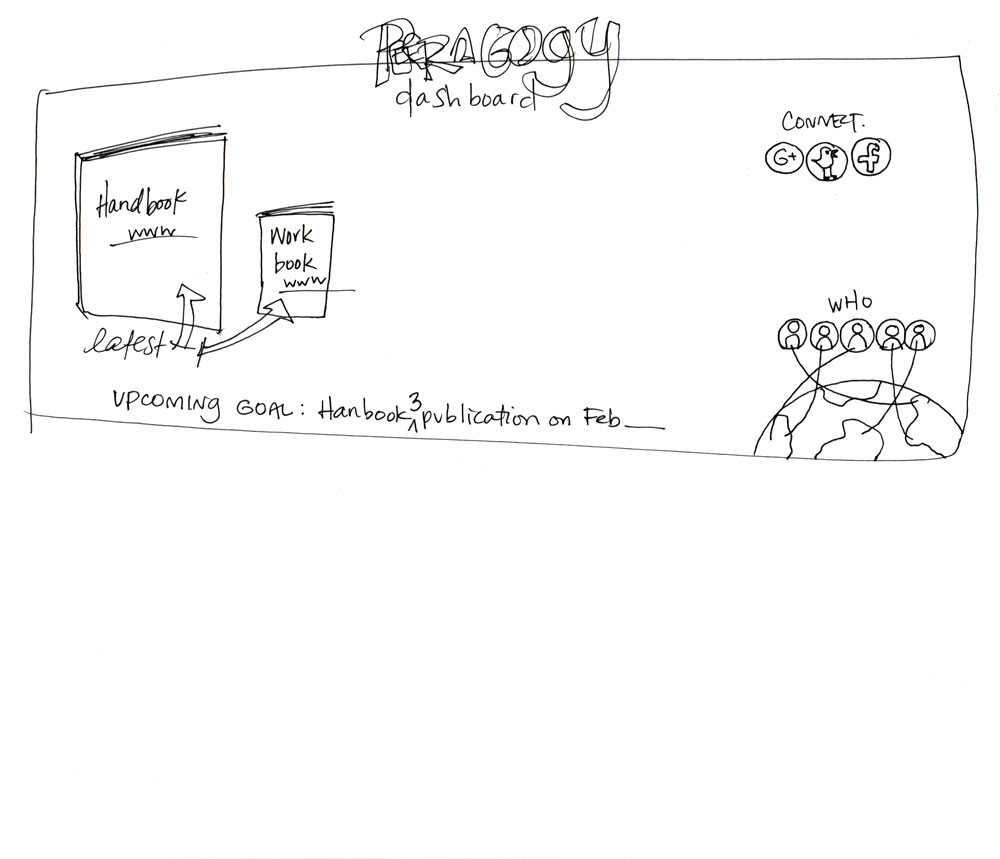
\includegraphics[width=\textwidth,trim=0mm 135mm 0mm 0mm,clip=true]{figures/peeragogy_dashboard_draft1/peeragogy_dashboard_draft1.jpg}
\caption{Design sketch for possible updated Peeragogy project dashboard (image by Amanda Lyons, used with permission).}
\end{figure}
